\chapter{Introduction}\label{chap:introduction}%
% Problem tanimi
% Neden cozmek istiyoruz
\section{Dictionaries}%
\label{sec:dictionaries}

Dictionaries are living records of a society's language usage.
Languages change over time, people adopt new words for new senses while others fall out of use.
Concepts appear as a result of technological advancements or social shifts, giving birth to new senses and words to define them.
Meanwhile, the term \emph{dictionary} is a broad one to define.
On its own, it brings forth the monolingual dictionary into consideration~\cite{sterkenburg_practical_2003}.
This type of dictionary presents words alongside their definitions following an alphabetical order.
The intention is to inform the user about the words~\cite{uzun_modern_2005}.
Other types of dictionaries vary with regard to their use case, target audience, and scope.
For instance, bilingual dictionaries present words alongside their translations in the target language, often used by language learners or translators.
Domain specific dictionaries list technical terms that target people who are familiar with the terminology.

The term that precedes the entries is called \emph{headword} or \emph{lemma}.
Usually, lemmas are the form of a word without inflections.
The sense they convey is as comprehensive as possible, reducing the number of otherwise redundant entries that would have been the derivatives of the unmarked form~\cite{ibrahim_usta_turkce_2006}.

Dictionaries also inform the user about how senses relate to each other.
\textbf{Polysemous} words share the same spelling while having related, often derivative meanings.
For example; under the entry for the term \emph{bank}, a definition might clarify the meaning \emph{financial institution} while another can define \emph{the building of a financial institution}.
In contrast, \textbf{homonymous} words have distinct meanings while having identical spellings through coincidence.
Formal definition of homonymy separates sound based and spelling based homonymy differently as homophones and homographs but for the purposes of our text based arguments, we do not delve into the specifics.
The \emph{bank of a river} is homonym to the given examples.
Homonyms are often shown in discrete blocks of descriptions.

\textbf{Synonymity} is another lexical relation we are interested in.
A word is synonymous to another if they share the same meaning but are not spelled alike, such as the terms \emph{right} and \emph{correct}.
However, synonymity is seldom shown in dictionaries.

% from dictionaries to multilingual web
Dictionaries take an immense amount of time and expertise to prepare.
We can talk about the examples after narrowing our scope down to the dictionaries that are still available today.
A survey by \textcite{uzun_1945ten_1999} notes that the first instalment of the modern Turkish dictionary, led by a team of experts, has taken over 6 years to prepare.
\textcite{kendall_forgotten_2011} talks about how Noah Webster, the writer of the \emph{An American Dictionary of the English Language} had to mortgage off his home in order to finish his project which took over 26 years.
The bulk of this effort is collecting documents and other written material in order to establish a \emph{corpus}~\cite{uzun_1945ten_1999}.
This endeavour is necessary since a corpus is crucial to create the vocabulary of a language.
Once the corpus is at hand, researchers can extract the lemmas.
The resulting wordstock is called the \emph{lexicon} of the language.

The internet radically changed the way researchers aggregate data.
The advancements in digital storage technology allowed the data to be persistent.
Improvements in networking ensured that people can share the volume of it among themselves.
With the popularization of social media, the internet generates everyday conversations at an unprecedented rate that researchers are using for natural language applications.
% TODO A reference here
Moreover,  efforts on open, collaborative, web based encyclopedias generate structured, multilingual data often used in machine translation and text categorization tasks.
% TODO A reference here
Once the cumbersome task of corpus attainment is now akin to web crawling.
With the digitized data, it was only natural for dictionaries to go digital as well since it's generally acknowledged that they are no longer viable if they are not electronic~\cite{sterkenburg_practical_2003}.

% start wordnets
\section{WordNet}% not sold on having 'wordnet' as a section
\label{sec:wordnet}
George A.\ Miller started the WordNet project in the mid-1980s.
On its early days, project members studied theories that were aimed towards enabling computers to understand natural language as intrinsically as humans do.
While working on then popular semantic networks and sense graphs, they have started something that will evolve into an expansive, influential resource~\cite{fellbaum_wordnet_1998}.

Traditional dictionaries are rigid, constrained by the nature of the printed form.
Today, people can browse WordNet via queries, like an online dictionary or a thesaurus.
Behind the scenes, a sprawling lexical database has relationship information for more than 117000 senses.
% wrong, actually has 117000 synsets, sense != synset?
Figure~\ref{fig:example_run} shows a brief result for the query string \enquote{run}.

\begin{figure*}[!hbp]
    \begin{center}
        {%
            \setlength{\fboxsep}{1pt}%
            \setlength{\fboxrule}{1pt}%
            \fbox{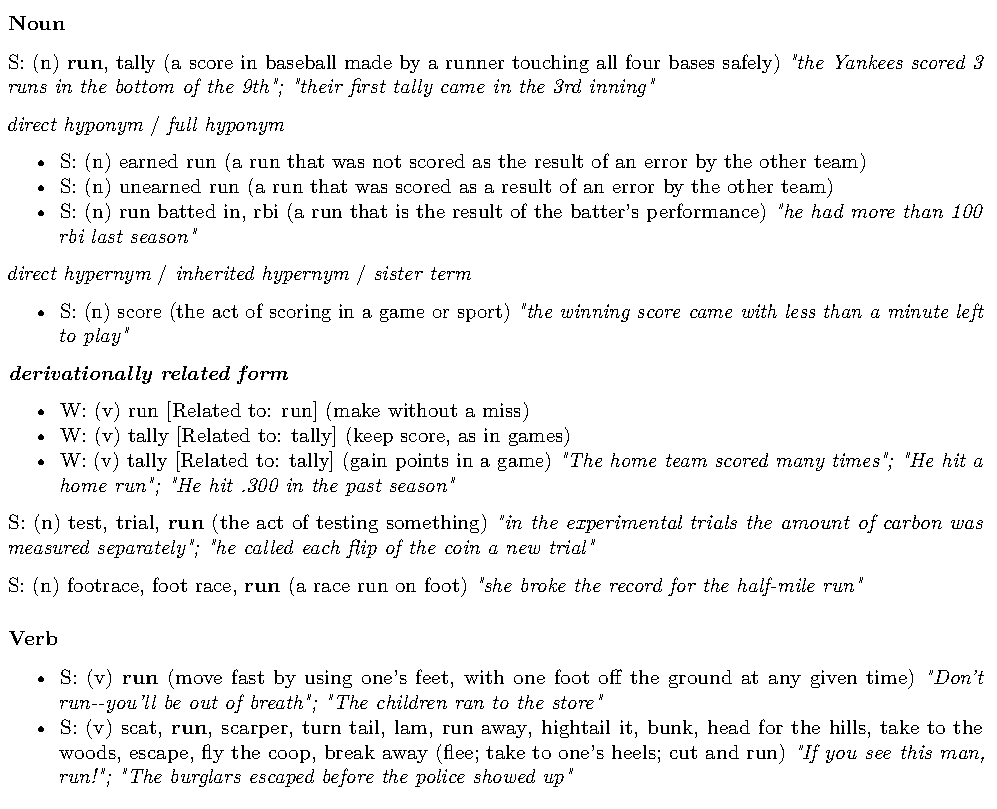
\includegraphics[page=1,width=\textwidth]{Figures/run_wordnet.pdf}}
        }%
        \caption{WordNet result for the query \enquote{run}, truncated for brevity.}\label{fig:example_run}
    \end{center}
\end{figure*}

WordNet lists terms, much like a traditional dictionary, alongside its polysemes but also their homonyms.
Additionally, there is a horizontal association; for any sense, the lemmas that share the row with the target term are synonyms.
Furthermore, synset terms can have one or more lexemes, not necessarily singular tokens.
This set of synonyms is aptly named \emph{synsets}.
An example synset is \{\emph{ledger}, \emph{account book} and \emph{book of account}\}.

A short description is also provided to clarify the meaning.
For the synset given above, the definition is; \enquote{a record in which commercial accounts are recorded}
These descriptions, hence the meanings for any synset is unique within the WordNet.
During this discussion, we have used sense and synset interchangeably.

WordNet also includes other relationships such as \emph{hypernymy} and \emph{hyponymy}, semantic relation of senses being type-of one another~\cite{miller_nouns_1990}.\footnote{not to be confused with homonymy}
For instance, the term \enquote{building} is a hyponym of \enquote{restaurant} since it encompasses a more general sense; the restaurant is type of a building.
While coffee shop is a hypernym to the restaurant since it is a more specific sense.

\begin{figure}[htbp]
    \centering
    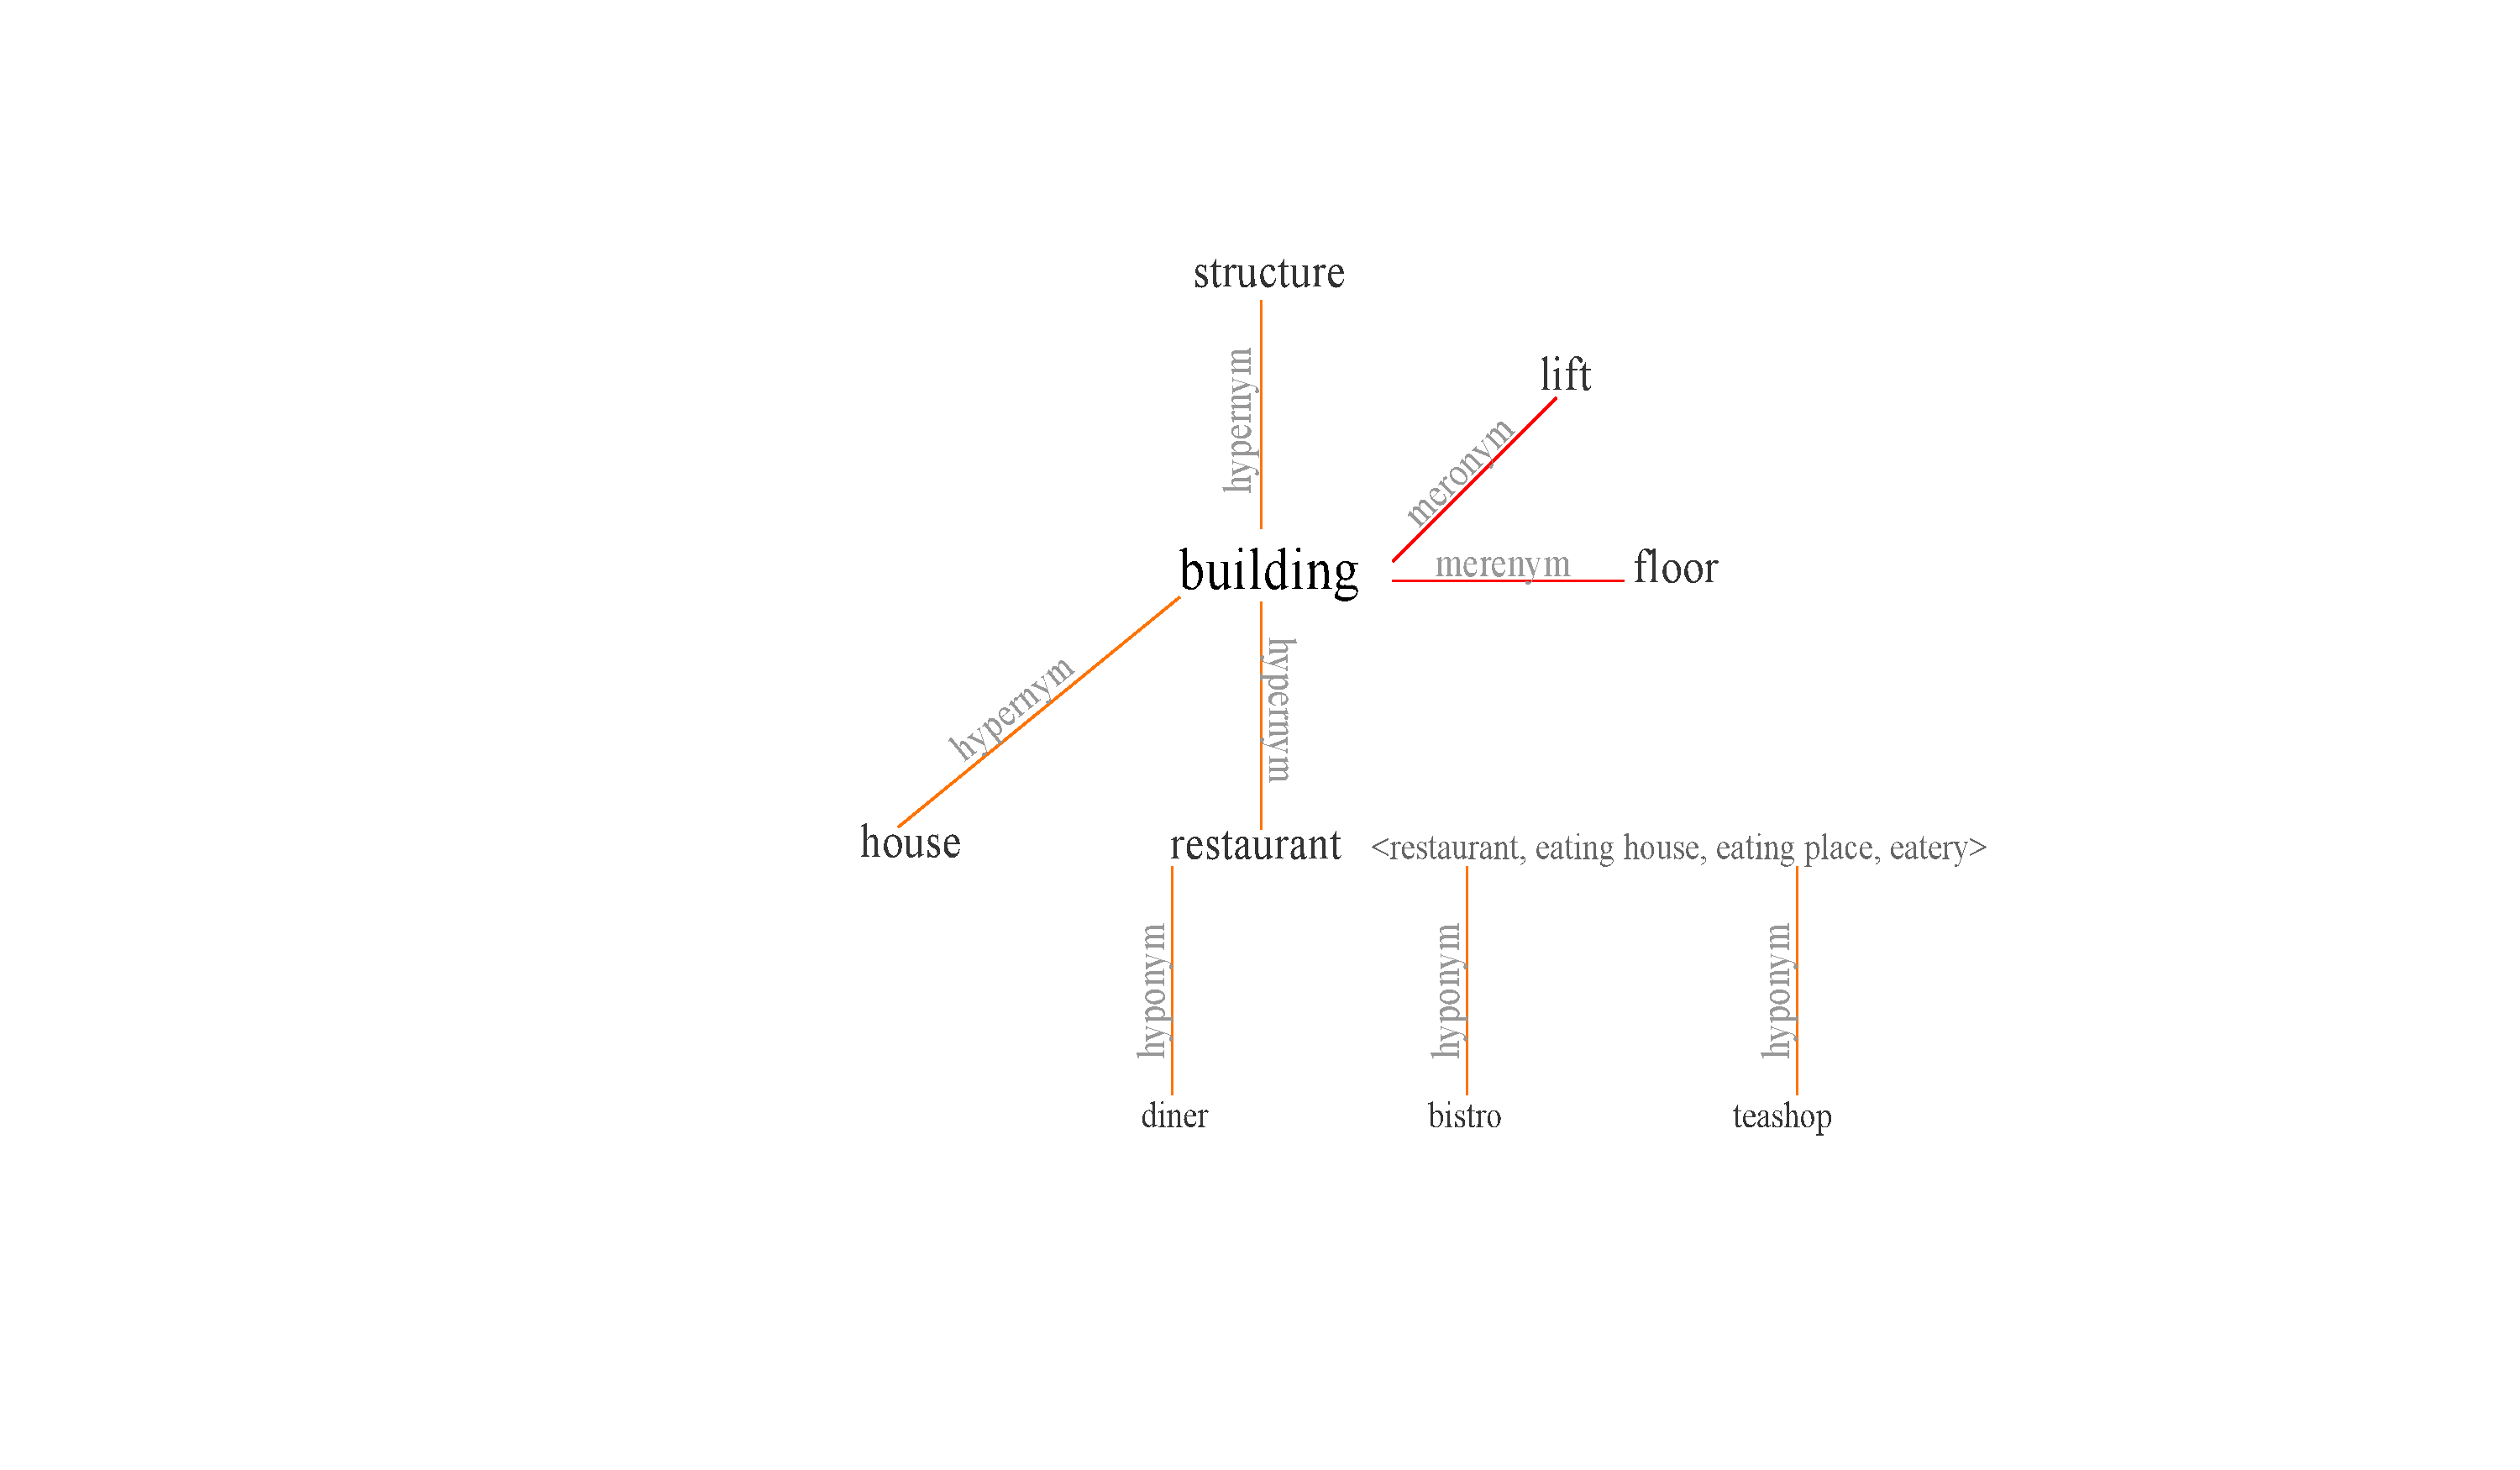
\includegraphics[page=1,width=\textwidth]{Figures/hyponym_hypernym.pdf}
    \caption{Example of a WordNet relationship graph. Hyponymy/hypernymy relations are shown from the hierarchy level of \emph{restaurant}}%
    \label{fig:hyponymy}
\end{figure}

One other relation is the meronymy, defined as a sense being part of or a member of another~\cite{winston_taxonomy_1987}.
Keeping to our building example, windows are meronym to buildings.
Other relationships exist but listing them is outside the scope of this thesis.
Bottom line is the effort that has gone through to map 117,000 senses according to different semantic relationships.
\textcite{sagot_building_2008} argue that the semantic relationships between senses are not tied to a specific language.
With this assumption at hand, we can infer the effort behind the WordNet does not need to be repeated but can be translated to other languages.

Since it's inception, other projects built lexical databases, using the same WordNet design.
\textcite{fellbaum_semantic_1998} talks about the correct terminology that we abide for the thesis; \enquote{As WordNet became synonymous with a particular kind of lexicon design, the proper name shed its capital letters and became a common designator for semantic networks of natural languages}.
Hence \emph{WordNet} refers to English Princeton WordNet, while \emph{wordnets} created for other languages are not stylized.

\section{Multilingual Wordnets}%
\label{sec:multilingual_wordnets}
Authorities list more than 7000\footnote{\url{https://www.ethnologue.com/statistics}} living languages but only 40\footnote{\url{https://w3techs.com/technologies/history_overview/content_language/}} of them have a sizeable presence on the internet.
Among this small fraction, English is the dominant language of the web.
English in not the centrepiece for natural language processing research because of any linguistic attribute.
It is simply the most abundant language on web, giving researchers data to work with.

Natural language processing library spaCy\footnote{\url{https://spacy.io/}} resorts to lemmatizations such as \emph{=PRON=} to denote pronouns in order to collapse the senses for \enquote{I} \enquote{you}, \enquote{them} etc.\@.
The sense and the accompanying word for the brother of a person's father or mother differs in Turkish, Danish, Chinese and Swedish among other languages while both collapse to \enquote{uncle} in English.
Studying other languages can provide insight towards concepts that are not present in English.

Translation, information transfer from foreign languages is a valid way of enriching a language's corpora; if a term that for a sense does not have a match in the target language, it is a good indication for the linguists of that language to look into their lexicons and work towards expanding it~\cite{ibrahim_usta_turkce_2006}.
Further research in the area contributes to languages other than English having access to tools that will incorporate them into the literature.

Open Multilingual WordNet~\cite{bond_survey_2012} set out to discover the effects related to the choice of license for wordnets.
Their criteria for usefulness is the number of citations a publication tied to the wordnet has gotten on literature.
They identified two major problems with the current distributions;
\begin{itemize}
    \item some projects have picked restrictive licenses, effectively barring access to their tools for research purposes.
    \item the structures of the wordnets are not standardized, creating additional cost for creating programs to parse and use the wordnets.
\end{itemize}
In order to overcome the standardization issue, \citeauthor{bond_survey_2012} have aligned the wordnets according to their English Princeton WordNet lemma ids and have written individual scripts to parse them.
They are currently hosting the results from a single source.\footnote{\url{http://compling.hss.ntu.edu.sg/omw/}}

With alignment information at hand, we have created our dataset that we will assume to be perfectly aligned; a golden corpus.
Among the 34 wordnets available on Open Multilingual WordNet, only 6 of them have gloss information available.
Given this thesis will only investigate the ability to map senses using definitions of the sense, we used the subset of Albanian~\cite{ruci_current_2008}, Bulgarian~\cite{simov_constructing_2010}, Greek~\cite{stamou_exploring_2004}, Italian~\cite{pianta_multiwordnet_2002}, Slovenian~\cite{fiser_slownet_2012} and Romanian~\cite{tufis_romanian_2008} wordnets.
Table~\ref{tab:summary_table} shows brief statistics about them.
We should note that the languages of the wordnets used in the thesis are all present in the 40 languages that have a significant presence on the internet that we have mentioned before.
We have constrained this study to use only the freely available wordnets and not considered wordnets that are gated behind restrictive licenses.
\begin{table}[htbp]
    \centering
    \begin{tabular}{llr}
        \toprule%
        \textbf{Name of the Project} & \textbf{Language} & \textbf{Number of Definitions} \\
        \midrule%
        Albanet & Albanian & 4681 \\
        BulTreeBank WordNet & Bulgarian & 4959 \\
        Greek Wordnet & Greek & 18136 \\
        ItalWordnet & Italian & 12688 \\
        Romanian Wordnet & Romanian & 58754 \\
        SloWNet & Slovenian & 3144 \\
        \bottomrule %
    \end{tabular}
    \caption{Summary of the Wordnets used.}%
    \label{tab:summary_table}%
\end{table}

\section{Thesis Goals}%
\label{sec:thesis_goals}
% TODO we assume word embeddings are interchangeable
% TODO return here

In this thesis, we will study the dictionary alignment problem.
It naturally arises on wordnet generation tasks when extend approach is used.
Wordnet generation as well as extend approach will be talked about in detail in Section~\ref{sec:approaches_in_wordnet_generation}.
It can be used in conjunction with word sense disambiguation frameworks to match the correct sense of a term across languages.

Two unsupervised approaches will be presented as an answer to dictionary alignment problem.
First one is the matching approach, in which the dictionary definitions across languages will be thought as nodes of a weighted bipartite graph.
By assigning appropriate weights to the edges with respect to distance between individual dictionary definitions, we hypothesize that there is a case where minimum flow is achieved between the disjoint dictionary sets.
The same case can also be stated as the case where the edge weights of the matching is maximum if a similarity metric is used to assign weights.

The second unsupervised approach will be a document retrieval approach, adapted on dictionary definitions.
An algorithm that works with the consideration of individual distances between words will be presented.

We will also look into an encoder using a neural network approach.
The encoder will be trained on a metric for determining if two sentences that were written in different languages entail the same sense.
The performance of the encoder will hopefully give us insight towards using a bag of words model of sentence representation, decoupled from syntax of the language can be viable for the task.

All in all, we will investigate the following research questions;
\begin{itemize}
    \item How feasible is it to align senses across languages using their dictionary definitions.
    \item Which state of the art algorithms is most suitable for the task.
    \item Which parameters should be taken into consideration while tackling this task
\end{itemize}

We will not train our own word embeddings but get existing models.
This highlights the major advantage of our approach;
current word embedding models are trained on billions of tokens to learn the distributional properties of the words.
Comparatively, dictionaries are short texts.
However, we can bring the word embeddings trained out of domain to solve in domain tasks.

\section{Thesis Outline}%
\label{sec:thesis_outline}

First, we present the most important preliminary to our study in Chapter~\ref{chap:background_n_related}, the word embeddings.
Word embeddings provided the crucial basis for out thesis.
Without relying on representing words in a multidimensional space, establishing distance formulation simply would not work.
So we report on the history of how this representations came about, present the current popular approaches to learning and distributing word embeddings and discuss the models we have chosen in detail.
Even though the presented approaches can work with any two pairs of dictionary definition collections, one practical use for this application using the alignment process to extend the semantic database WordNet.
We report on approaches on wordnet generation using the previous works that created wordnets.
Other related work on representing senses are briefly discussed on Chapter~\ref{chap:background_n_related} as well.

In order to address our research questions, we have looked into approaches that can be broken down into 3 separate categories.
\begin{enumerate}
    \item Matching approach
    \item Retrieval approach
    \item Supervised approach
\end{enumerate}

Chapter~\ref{chap:unsupervised_matching} is concerned with the exploration of the unsupervised matching techniques.
Here we will present how dictionary alignment problem can be cast as a bipartite graph matching problem and report on our approach using linear programming.

We will handle dictionary alignment problem using state of the art document retrieval algorithms in Chapter~\ref{chap:retrieval}.
We will delve into the details of how the current approaches leverage word embeddings in order to represent words as probability distributions that lie on a multidimensional simplex.
Furthermore, we will explain the algorithms behind how efficient distance calculations can be achieved in this problem setting.

Chapter~\ref{chap:supervised_validation} is reserved for our supervised approach.
Given two definitions collections that we accept as perfectly aligned, we will investigate if an encoder can learn the semantic similarity as a function given positive and negative examples.
In order to present our problem, we will report on the current state of the art approach on semantic similarity and the neural network model that forms the basis of said approach.

Since our thesis is heavily concerned with investigating the best approach for the task at hand, we collected all our results in Chapter~\ref{chap:experiments_and_evaluation}.
By presenting all results from a single place, we hope to give a complete picture on how we have attacked the dictionary alignment task, which approaches performed better against others and the findings that emerged within the results.
Details concerning our implementation, how we obtained the aligned corpora and the word embeddings that share the same latent space are explained in Chapter~\ref{chap:experiments_and_evaluation} as well.

Last but not least, we will conclude our thesis in Chapter~\ref{chap:conclusion} with an overall look on our findings and the future work that we would like to study next.
